\section{Ejercicio 1}
    % 1. Describir detalladamente el problema a resolver dando ejemplos del mismo y sus soluciones.
    \subsection{Descripción del problema}
        Gokú debe entrenar un ejército de $N$ guerreros para enfrentarse a Majin Boo. Para lograr ese objetivo, desea organizar peleas entre sus luchadores. En cada pelea, los guerreros serán divididos en dos bandos que pelearán entre sí. El objetivo es que, para cualquier par de luchadores, haya al menos una pelea en la que se encuentren en bandos distintos. Al mismo tiempo, el número total de peleas debe ser el mínimo necesario.

        La resolución del problema consiste en elaborar un programa que recibe como entrada el valor de $N$, y devuelve la cantidad mínima de peleas que deben llevarse a cabo para cumplir el cometido de Gokú y a continuación, por cada una de las peleas, una línea indicando el bando al que pertenece cada uno de los luchadores durante la misma. De haber más de una solución posible, puede devolverse cualquiera de ellas.

        Por ejemplo, si el programa recibe como entrada el valor \texttt{8}, cualquiera de las siguientes tres salidas sería correcta:

        \begin{center}\begin{tabular}{l @{\hskip 2em} | @{\hskip 2em} l @{\hskip 2em} | @{\hskip 2em} l}
            \texttt{3}               & \texttt{3}  &              \texttt{3}               \\
            \texttt{1 1 1 1 2 2 2 2} & \texttt{1 1 2 2 2 1 2 1} & \texttt{2 1 1 1 2 1 2 2} \\
            \texttt{1 1 2 2 1 1 2 2} & \texttt{1 1 2 1 2 2 1 2} & \texttt{1 2 1 1 2 2 2 1} \\
            \texttt{1 2 1 2 1 2 1 2} & \texttt{2 1 2 1 1 1 2 2} & \texttt{1 1 2 1 2 2 1 2} \\
        \end{tabular}\end{center}

    % 2. Explicar de forma clara, sencilla, estructurada y concisa, las ideas desarrolladas para la resolución del problema. Utilizar pseudocódigo y lenguaje coloquial (no código fuente). Justificar por qué el procedimiento resuelve efectivamente el problema.
    \subsection{Solución propuesta}
        La idea central en la resolución del problema fue la siguiente: en cada pelea, Gokú debe tratar de que luchen entre sí la mayor cantidad posible de guerreros que no se hayan enfrentado en una pelea anterior. En particular, en la primera pelea, querrá dividir los bandos de forma tal que luchen entre sí tantos guerreros como sea posible.

        La idea intuitiva es que la solución óptima consiste en minimizar la diferencia entre las cantidades de guerreros de ambos bandos. Por ejemplo, si Gokú pone en un bando a un único guerrero y en el otro a los $N - 1$ guerreros restantes, los pares de guerreros que se enfrentarán en esa pelea serán $N - 1$, ya que todos los guerreros del segundo bando lucharán contra el que quede en el primero, pero nunca pelearán entre sí. Si, en cambio, decide poner $2$ guerreros en un bando, cada uno de ellos se enfrentará con los $N - 2$ del bando opuesto. Así, la cantidad de parejas de guerreros que se enfrenten será $2 (N - 2)$, mejorando el resultado anterior.
        
        En general, el conjunto de pares de guerreros que se enfrentan en cada pelea es el producto cartesiano de ambos bandos. Si el primer bando tiene $k$ guerreros, el otro tendrá $N - k$, por lo que el cardinal de este producto será $N (N - k) = N^2 - Nk$. Es sencillo ver que este producto es máximo cuando $k = \frac{N}{2}$.

        A la hora de resolver el problema, se utilizó la técnica de programación \emph{dividir y conquistar}, volcando de forma casi directa el razonamiento recién expuesto. Si se deja momentáneamente de lado el requerimiento de que la cantidad de peleas efectuadas sea mínima, el problema puede resolverse de esta forma:

        \begin{enumerate}
            \item Se comienza dividiendo a los peleadores en dos subconjuntos $A$ y $B$, que constituirán los bandos que se enfrentarán en la primera pelea.
            \item A continuación, hay que asegurarse de que los guerreros que quedaron en el mismo subconjunto se enfrenten en las peleas posteriores. Esto puede hacerse aplicando el algoritmo de forma recursiva sobre ambos subconjuntos. Así se obtiene, para cada subconjunto, una serie de \emph{subpeleas} que garantiza que todo par de peleadores se enfrenta al menos una vez.
            \item Se concatenan las \emph{subpeleas}, haciendo que la $i$-ésima \emph{subpelea} del subconjunto $A$ ocurra simultáneamente con la $i$-ésima \emph{subpelea} del subconjunto $B$. Si en uno de los subconjuntos deben realizarse más \emph{subpeleas} que en el otro, resulta indistinto en qué bando se encuentran durante las mismas los peleadores del otro subconjunto.
        \end{enumerate}

        Aplicando estos pasos e ignorando el requisito de que la cantidad de peleas sea la mínima posible, Gokú podría obtener, a partir de la entrada $N = 10$, el resultado que se muestra en la Figura \ref{fig:ej1-non-optimal-example}.

        \begin{figure}[h]
          \centering

          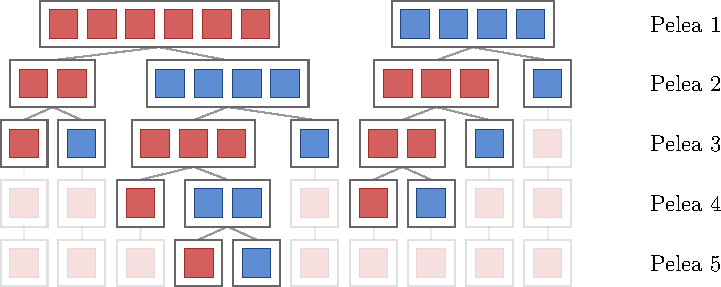
\includegraphics{imagenes/ej1-non-optimal-example.pdf} \vspace{1em} \\

          \caption{Ejemplo de solución (no óptima) para el caso $N = 10$. Son necesarias 5 peleas.}
          \label{fig:ej1-non-optimal-example}
        \end{figure}

        Desde luego, nada nos garantiza que, en cada paso de la recursión, Gokú haya tomado las decisiones óptimas. ¿Podría lograrse que todos los peleadores se enfrenten en una menor cantidad de peleas? Aplicando las ideas antes expuestas, y haciendo que en cada paso de la recusión los subconjuntos $A$ y $B$ tengan $\frac{N}{2}$ guerreros cada uno, se obtiene una mejor solución, como muestra la Figura \ref{fig:ej1-optimal-example}.

        \begin{figure}[h]
          \centering

          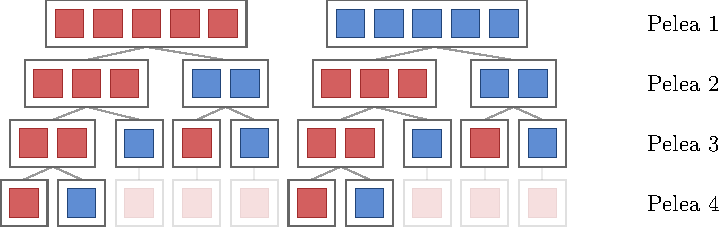
\includegraphics{imagenes/ej1-optimal-example.pdf} \vspace{1em} \\

          \caption{Ejemplo de solución óptima para el caso $N = 10$. Solo hacen falta 4 peleas.}
          \label{fig:ej1-optimal-example}
        \end{figure}

        

    % 3. Deducir una cota de complejidad temporal del algoritmo propuesto y justificar por qué el algoritmo cumple la cota dada. Utilizar el modelo uniforme.
    \subsection{Complejidad teórica}
         
        Para justificar la complejidad usaremos el Teorema Maestro 
        \[T(n) = \begin{cases} 2T(\frac{n}{2}) + f(n) &  n > 1 \\
                                \theta(1) & n = 1    \end{cases} \]
        Trivialmente en el caso que sea n sea 1, se ve que su complejidad es $\theta(1)$ .El costo de la funcion  $f(n)$ es $\theta(n)$ , dado que el costo de armar la pelea es  $\theta(n)$  .
        Dado que 2 es la cantidad des subproblemas a resolver y tambien las particiones y n es el costo de cada paso en la recursión , el algoritmo cae en el segundo caso , entonces la complejidad es de $ n log n$.



    % 4. Dar un código fuente claro que implemente la solución propuesta. Se deben incluir las partes relevantes del código como apéndice del informe impreso entregado.

    % 5. Realizar una experimentación computacional para medir la performance del programa implementado. Usar un conjunto de casos de test en función de los parámetros de entrada, con instancias aleatorias e instancias particulares (de peor/mejor caso en tiempo de ejecución, por ejemplo). Presentar en forma gráfica una comparación entre los tiempos medidos y la complejidad teórica calculada y extraer conclusiones.
    \subsection{Experimentación}

	A la hora de medir el rendimiento del algoritmo y confirmar la complejidad
	teórica se tuvieron que considerar varios aspectos tales que los
	resultados de la experimentación reflejaran lo mejor posible su
	comportamiento.

	Dado que el problema consiste en una única entrada, los casos de prueba
	posibles se reducen al conjunto de los números enteros positivos. Como la
	complejidad temporal del algoritmo es $\theta(Nlog(N))$, no hay un peor
	y mejor escenario, por lo tanto no es necesario establecer condiciones sobre
	la entrada.

	El experimento consiste en la medición de los tiempos de ejecución para
	entradas cada vez más grandes. A continuación se describen las condiciones aplicadas
	para el mismo:

	\begin{itemize}
		\item{Como entrada se utilizó $N = 2^{k}$ con $0 < k < 24.$}
		\item{Por cada $N$, se repitió 10 veces la medición y se calculó un
			promedio.}
		\item{Sólo se midió el costo temporal de generar la solución, no
			de lectura y escritura del problema.}
		\item{Para la medición del tiempo se utilizó la librería \texttt{chronos}
			con unidad de tiempo en nanosegundos.}
	\end{itemize}

	De estos puntos, cabe destacar la elección de potencias de dos como
	entrada. Esta decisión surge del hecho de que en valores pequeños las
	mediciones de tiempo son más sensibles a perturbaciones del sistema en el
	que están corriendo. Al elegir $N = 2^{k}$ como entrada tenemos que para los
	primeros valores de $k$, los $N$ resultantes se encuentran relativamente
	concentrados, logrando así un muestreo que caracterice mejor estos valores.
	A medida que se aumenta el $k$, obtenemos valores de entrada más espaciados
	con tamaños donde el ruido introducido por el sistema es despreciable.

	Los resultados obtenidos fueron los siguientes:

	\newcommand\constante{30}
	\begin{figure}[H]
		\centering
		\caption{}
		\label{fig:tiempo_base}
		\begin{tikzpicture}
			\begin{axis}[
					title={},
					xlabel={Tamaño de entrada ($N$)},
					ylabel={Tiempo de ejecución (nanosegundos)},
					scaled x ticks=false,
					scaled y ticks=false,
					enlargelimits=0.05,
					width=0.5\textwidth,
					height=0.5\textwidth,
					legend pos=south east,
					legend cell align=left,
					xmin=1
				]
				\addplot[color=black] table[x index=0,y index=1]{../exp/kaioKenOutput};
				\addplot[color=red] table[x index=0, y expr={x*ln(x)*\constante}]{../exp/kaioKenOutput};
				\legend{$T$, $c*N*log(N)$}
			\end{axis}
		\end{tikzpicture}
	\end{figure}

	En la Figura \ref{fig:tiempo_base} se puede observar como la curva generada por el
	tiempo de ejecución puede ser acotada para un $c$ fijo por una función
	$c*N*log(N)$. Para ratificar esta observación se procede dividiendo cada $T$
	por su respectivo $N$ con la intención de generar una curva de forma
	logarítmica.

	\begin{figure}[H]
		\centering
		\caption{}
		\label{fig:tiempo_sobre_n}
		\begin{tikzpicture}
			\begin{axis}[
					title={},
					xlabel={Tamaño de entrada ($N$)},
					ylabel={Tiempo de ejecución (nanosegundos)},
					scaled x ticks=false,
					scaled y ticks=false,
					ymax=500,
					enlargelimits=0.05,
					width=0.5\textwidth,
					height=0.5\textwidth,
					legend pos=south east,
					legend cell align=left,
					xmin=1
				]
				\addplot[color=black] table[x index=0,y index=2]{../exp/kaioKenOutput};
				\addplot[color=red] table[x index=0, y expr={ln(x)*\constante}]{../exp/kaioKenOutput};
				\legend{$\frac{T}{N}$, $c*log(N)$}
			\end{axis}
		\end{tikzpicture}
	\end{figure}

	Con la Figura \ref{fig:tiempo_sobre_n} se corrobora lo previsto, ya que
	efectivamente se puede apreciar cómo con la misma constante $c$ se puede
	acotar por una función $c*log(N)$.

	\begin{figure}[H]
		\centering
		\caption{}
		\label{fig:tiempo_sobre_n_log_n}
		\begin{tikzpicture}
			\begin{axis}[
					title={},
					xlabel={Tamaño de entrada ($N$)},
					ylabel={Tiempo de ejecución (nanosegundos)},
					scaled x ticks=false,
					scaled y ticks=false,
					ymin=0,
					ymax=150,
					enlargelimits=0.05,
					width=0.5\textwidth,
					height=0.5\textwidth,
					legend pos=south east,
					legend cell align=left,
					xmin=1
				]
				\addplot[color=black] table[x index=0,y index=3]{../exp/kaioKenOutput};
				\addplot[color=red] table[x index=0, y expr={\constante}]{../exp/kaioKenOutput};
				\legend{$\frac{T}{N*log(N)}$, $c$}
			\end{axis}
		\end{tikzpicture}
	\end{figure}

	Finalmente, en la Figura \ref{fig:tiempo_sobre_n_log_n} se tiene que
	$\frac{T}{N*log(N)}$ converge a una constante que es acotada por el $c$
	utilizado en las figuras anteriores.

	Es así como se llega a la conclusión de que efectivamente la complejidad
	temporal de la solución desarrollada coincide con la complejidad teórica estipulada.

	Para reproducir los datos utilizados basta con ejecutar \texttt{KaioKenSolver
	-p}.
